% !TEX root =  ../../thesis.tex

\chapter{Bayesian linear mixed effects model}
\label{ch : blmm}

\section{Introduction to linear mixed model}
\label{sec : lmm}
A linear mixed effects model, also known as linear mixed model(LMM) is a statistical model for data which is hierarchical in structure. The specialty of the models is that apart from the fixed effects, they also model the correlation between the observations falling in the same group at a certain level in the hierarchy. The correlation is modeled using the random effects and the response is modeled as a linear function of both fixed and random effects.\\

There are many synonymous terminologies for data sets which are hierarchical in nature albeit with subtle nuances differentiating them. In this thesis our focus will be on Longitudinal data sets. A longitudinal data set is the one where multiple observations are collected from subjects at different points in time. For e.g. measurement of Hemoglobin of 20 patients with observations taken every month for a period of 24 months. Since the observations collected from a subject will be correlated a linear model will not be useful because of the restrictions it imposes on the covariance structure.

\subsection{LMM definition}
\label{subsec : lmm_definition}
Following the notations from \citet{lesaffre_bayesian_2012}, the LMM for the observations of the $i^{th}$ subject among the $n$ subjects is given by

\begin{equation}
\label{eq : lmm_definition}
\boldsymbol{y}_i = \boldsymbol{X}_{i}\boldsymbol{\beta} + \boldsymbol{Z}_{i}\boldsymbol{b}_{i} + \boldsymbol{\varepsilon}_{i}
\end{equation}

where $1 \le i \le n$,\\
$\boldsymbol{y}_i = {(y_{i1}, y_{i2}, \ldots, y_{im_i})}^T$ is a vector of observations for the $i^{th}$ subject taken at $m_i$ time points,\\
$\boldsymbol{X}_i = {(\boldsymbol{x}_{i1}^T, \boldsymbol{x}_{i2}^T, \ldots, \boldsymbol{x}_{im_i}^T)}^T$ is the $m_i \times (d+1)$ design matrix for the $i^{th}$ subject,\\
$\boldsymbol{\beta} = {(\beta_0, \beta_1, \ldots, \beta_d)}^T$ is a $(d+1) \times 1$ vector of fixed effects with $\beta_0$ being the intercept,\\
$\boldsymbol{Z}_i = {(\boldsymbol{z}_{i1}^T, \boldsymbol{z}_{i2}^T, \ldots, \boldsymbol{z}_{im_i}^T)}^T$ is the $m_i \times q$ design matrix of covariates multiplying the random effects,\\
$\boldsymbol{b}_i = {(b_{0i}, b_{1i}, \ldots, b_{(q-1)i})}^T$ is a $q \times 1$ vector of random effects with $b_{0i}$ being the random intercept. The random effects $\boldsymbol{b}_i \sim N_q(\boldsymbol{0}, G)$ with $G$ being the $q \times q$ covariance matrix,\\ 
$\boldsymbol{\varepsilon}_{i} = {(\varepsilon_{i1}, \varepsilon_{i2}, \ldots, \varepsilon_{im_i})}^T$ is a $m_i \times 1$ vector of measurement errors. The errors $\boldsymbol{\varepsilon}_{i} \sim N_{m_i}(\boldsymbol{0}, R_i)$ with $R_i$ being the $(m_i \times m_i)$ covariance matrix of errors,\\

The errors $\boldsymbol{\varepsilon}_{i}$ and the random effects $\boldsymbol{b}_i$ are assumed to be independent. $R_i$ is usually a diagonal matrix of the form $\sigma^2I_{m_i}$. While one might only model the correlation between the observations of a subject using random effects, it is also possible to model the serial correlation component.

\section{Motivation for Bayesian linear mixed model}
\label{sec : blmm}
One of issues with the frequentist LMM is that while the parameters in matrices $G$ and $R_i$ are estimated using ML/REML only a point estimate is further used in estimation of fixed effects(see \cite[chap. 5]{verbeke_linear_2009}). Hence the uncertainty in estimation of random effects is ignored. Although frequentist inference approaches try to mitigate this issue by modifying the distributional assumptions of the test statistic \citep[pg. 56]{verbeke_linear_2009}, a bayesian approach considers the variability in parameter estimates in the first place. A similar problem occurs in the estimation of $\boldsymbol{b}_i$. The frequentist strategy is to use Empirical bayes estimates where the the posterior distribution of random effects uses point estimates of parameters in matrices $G$ and $R_i$. Thus the uncertainty in estimation is ignored. On the other hand the bayesian approach averages out over the entire posterior distribution of the hyperparameters to obtain the posterior $p(\boldsymbol{b}_i|\boldsymbol{y})$. In light of these reasons, in this thesis we will model our data using Bayesian linear mixed models.\\

The Bayesian linear mixed model or BLMM can be obtained by assigning a distribution to all the parameters involved in a LMM. This means that for the model presented in section \ref{subsec : lmm_definition} we will have a prior distribution for the following:
\begin{itemize}
\item $\sigma^2 \sim p(\sigma^2)$
\item $\boldsymbol{\beta} \sim p(\boldsymbol{\beta})$
\item $G \sim p(G)$
\end{itemize}

\section{Motivation for mixture of random effects}
As we saw above the random effects are assumed to be multivariate normally distributed. It could be too strong an assumption though in certain cases. A classical example of it are the longitudinal studies where at any time point we would like to categorize subjects in groups. For e.g. group with a high risk of having a certain disease in future vs. group with a low risk. While in retrospective studies it is quite easy as we know exactly which patients were diagnosed with the disease and which were not. However in a study where we would like to categorize patients into different groups well before diagnosis this could be difficult. Here is a toy example for it. Imagine that in longitudinal study we are measuring a response $Y$ which is an indicator of a disease. Assume that from a previous study it is known that patients which are in high risk group for the disease tend to have a higher response $Y$ during all times. Also assume that the trend of $Y$ over time remains the same for both groups otherwise. Figure \ref{fig : random_slope_dummy_data} shows individual profiles of subjects from a simulated dataset. Looking at this plot we can say that a random intercept component will be enough to model individual profiles. Since we will not be knowing which patient belongs to which group, this heterogeneity can be appropriately modeled by considering that the random intercept is a mixture of two normal components.\\

\begin{figure}
	\centering
	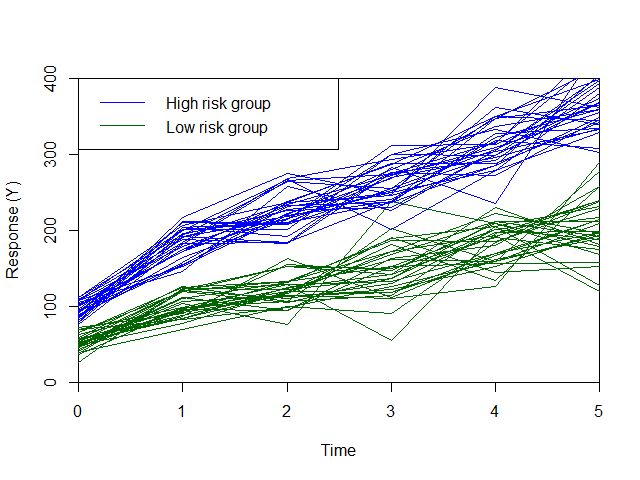
\includegraphics[scale=0.5]{mainmatter/chapter_3_blmm/random_slope_dummy_data.png}
	\caption{Individual profiles of 30 subjects from each group.}
	\label{fig : random_slope_dummy_data}
\end{figure}

In a LMM is quite common to use histogram of Empirical Bayes estimates of random effects to detect groups of individuals. However \citet{verbeke_linear_1996} have shown that if the prior is misspecified(for e.g. if in our example we use a univariate normal distribution), then the histogram of estimates of random effects will be shrunk towards the prior distribution. Thus it would be impossible to classify the subjects into different categories based on empirical bayes estimates of random effects as they are incorrect. A solution to this problem is using a mixture of Gaussian components for random effects distribution. Such a linear mixed model is termed as a Heterogeneity model.

\subsection{Bayesian heterogeneity model}
\label{subsec : bhtge}
The formal definition of a Bayesian heterogeneity model can be given by extending the Bayesian linear mixed model definition given in section \ref{sec : blmm}. Since, now the random effects have a Gaussian mixture distribution we will use the following notation to express the distribution mathematically.

$$\boldsymbol{b}_i \sim \sum_{k=1}^{K} \eta_k N_q(\boldsymbol{b}_k^C, G_k)$$\\
where $\boldsymbol{b}_k^C$ and $G_k$ are the mean vector and covariance matrices for the $k^{th}$ component in the mixture distribution respectively. The vector $\boldsymbol{\eta} = (\eta_1, \eta_2, \ldots, \eta_K)$ is the weight distribution for the component densities. The vector $\boldsymbol{S}=(S_1, S_2, ..., S_n)$ represents the allocation vector for all of the subjects. Since we are following the bayesian paradigm, in addition to prior distribution for $\boldsymbol{\beta}$ and $\sigma^2$ we also have prior for $\boldsymbol{\nu} = (\boldsymbol{b}_1^C, \boldsymbol{b}_2^C, \ldots, \boldsymbol{b}_K^C, \boldsymbol{\eta}, G_1, G_2, \ldots, G_K)$.